\documentclass[12pt]{article}
\usepackage[utf8]{inputenc}
\usepackage{booktabs}
\usepackage{multirow}
\usepackage{multicol}
\usepackage{rotating}
\usepackage{bigstrut}
\usepackage{tabularx}
\usepackage{prettyref}
\usepackage{setspace}

%% fonts
\usepackage[utopia]{mathdesign}
\usepackage[scaled=.95]{inconsolata}

%% page margins, inter-paragraph space and no chapters
\usepackage[margin=1in]{geometry}
\setlength{\parskip}{0.5em}
\renewcommand{\thesection}{\arabic{section}}

%% bibliography
%\usepackage[american]{babel}
%\usepackage{csquotes}
%\usepackage[style=apa,natbib=true,backend=biber]{biblatex}
%\DeclareLanguageMapping{american}{american-apa}
%\addbibresource{EITC.bib}

%% For actual bib
\usepackage{natbib}
\bibpunct{(}{)}{,}{author-year}{}{,}

%% Fuck with the title
\makeatletter
\renewcommand{\maketitle}{\bgroup\setlength{\parindent}{0pt}
\begin{flushleft}
  \textbf{\@title}

  \@author
\end{flushleft}\egroup
}
\makeatother

%% for memisc
\usepackage{booktabs}
\usepackage{dcolumn}

%% define a dark blue
\usepackage{color}
\definecolor{darkblue}{rgb}{0,0,.5}

%% hyperlinks to references
\usepackage{hyperref}
\hypersetup{colorlinks=true, linkcolor=darkblue, citecolor=darkblue, filecolor=darkblue, urlcolor=darkblue}

\author{Adam Olson\\University of Minnesota\\ \today}
\title{Dissertation Proposal Draft}
\date{February 9, 2014}

\begin{document}
\maketitle

\section{Introduction}
Most scholars who study comparative welfare states refer to the United States as exceptional because they believe any welfare state the United States had was less generous, developed later, and was smaller than welfare states in comparable developed countries (See especially \citealt{andersen1990}). In a very well received challenge to this conventional wisdom, \citet{hacker2002} pointed out, the ``welfare state'' is a contested idea both among political activists and scholars and that not every country provides social policy in a uniform manner. Since then, scholars including Jacob Hacker, Christopher Howard, and others have made a compelling case that what ``is exceptional about the American welfare state is not the level of spending but the source'' of spending \citep[pg. 7]{hacker2002}.

To that point, two prominent forms of social policy in the the United States are visible welfare programs and hidden welfare programs. Visible welfare programs are generally, though now always, considered the `traditional' programs that most people view as welfare programs in the United States, such as Medicare or Social Security. These are programs that are generally well known to politicians, interest groups, and the mass public. Traditionally, these are the programs which scholars refer to when they discuss measurements such as welfare effort or welfare spending - they are apparent attempts by the government to alleviate some socially undesirable problem such as poverty or hunger. Even though these traditional programs are what most scholars mean when they say visible welfare, there is wide variation in the programmatic components of these policies. They include both the major entitlements that we all know about, like Social Security, but also many of the means-tested programs as well such as Temporary Assistance for Needy Families, or the Supplemental Nutrition Assistance Program.

Hidden welfare programs, also known as the hidden welfare state, distribute benefits through the tax code as tax expenditures and other ways and is less obvious than the more visible parts \citep{howard1997}.\footnote{A more legalistic definition of tax expenditures is provided in the the Congressional Budget and Impoundment Control Act of 1974 as ``revenue losses attributable to provisions of the Federal tax laws which allow a special exclusion, exemption, or deduction from gross income or which provide a special credit, a preferential rate of tax, or a deferral of tax liability.''} One prominent example of a hidden welfare program is the Home Mortgage Interest Deduction which was created in 1913 to encourage home ownership and cost the federal government around 100 billion dollars in 2010. This type of welfare through the tax code cost the federal government 1.1 trillion dollars in 2013 which by some estimates is more than was spent on visible welfare programs \citep{omb2013}. Whereas, elderly Americans can apply for social security once they turn 62 and receive a check each month, the hidden welfare state is largely administered through the tax code without much bureaucratic overhead like with Social Security. Like in the visible welfare state, the government tries to alleviate social ills such as poverty or lack of housing (through the Earned Income Tax Credit and the Home Mortgage Tax Decution respectively), but it does so in a way that is not evident to most people and generally uses less obvious policy making processes \citep{mettler2011}. 

While our understanding of the hidden welfare state and political aspects of American social policy has increased overall due to recent research, there remain two gaps in the literature. The first major gap in this type of policy making literature is its inattention to the role of congressional behavior. Research on the American welfare state is strangely devoid of insight from the voluminous literature on congressional policy making. Political science has tremendous insight as to the role congressional parties, divided government, congressional committees, elections and many other facets of congressional life have on the behavior of individual MCs and Congress as a whole. While Congress often plays a staring role in scholarly accounts of social policy creation, this research seldom formally incorporates scholarly insight produced by congressional scholars. By applying some of the specific hypotheses outlined by congressional scholars to the historical creation and subsequent development of the American welfare state, we will be able to see how different congressional politics create different policy outcomes and develop a more dynamic set of predictions for when one type of social policy is created or advanced over another.	


Second, previous traditional welfare literature has studied traditional welfare programs largely in isolation from non-traditional programs. This necessarily produces an incomplete story in trying to understand the politics of American social policy on a broader level. Both visible and hidden programs seek to alleviate some sort of social ill and while the politics that go into producing a policy or the politics that the policy will produce may differ, policies in the same sphere should be examined in relation to one another. For example, the United States has several different policies which attempt to provide easier access to housing. Home owners can deduct large parts of their mortgage interest from their federal income tax, the government also provides vouchers to help subsidize rent, and in some cases even provide housing itself. How did America develop a housing policy which incorporates both indirect and direct spending? By examining both indirect and direct programs with similar programmatic goals we can understand how the politics of indirect policies are both similar and different from visible programs in such a way that increases our understanding of American social policy creation and development and the American welfare state overall.

In addition to the two gaps, this dissertation builds on trends that already existed with the idea that policymaking is an iterative process that involves both a creation component \emph{and also} a persistence component. After a policy is created, it has the potential to be expanded or retrenched by enterprising members of Congress (MCs) or bureaucrats. A policy that was created fifty years ago may look very different looks today because of subsequent reforms. This intersects with the second gap of not considering visible and hidden policies together as a visible policy may be retrenched even while a very similar hidden policy is expanded. Policy affect politics and the tools used to create policy have co-evolved programmatically and politically \citep{schattschneider1960, skocpol1995}.  Historically there has been attention paid to an individual policy's entire life, including after initial passage (see especially \citealt{derthick1979, hacker2002}), but by examining a group of policies, both at inception, and through subsequent development, we can deepen our understanding of the policy process.

Broadly, this dissertation asks how the United States came to rely on a mix of visible and hidden policies to provide social policy. In pursuing that question, I will draw heavily on the congressional institutions and behavior literature in formulating casual hypotheses. Additionally, it will answer why a legislator utilizes one policy making tool over another to advance their policy goals and discuss how different interests shape legislation. Consequently, this dissertation will be able to examine how individual programs are created \emph{and} persist vis-a-vis each other. The juxtaposition of the traditional American welfare state literature, hidden welfare state literature, and the congressional literature will drastically improve our understanding of how policy is created and changed  based on changing structural and ideological constraints.

\section{American Social Policy Development}

The American welfare state literature is rich and well developed, not only in descriptive accounts but also its theories of policy development. Broadly in this section, I discuss both of those parts. In the first subsection, I describe the American welfare state, focusing on the types of the mechanisms the government uses to provide social policy. In the second subsection, I outline the traditional hypotheses of social policy making in the United States and then apply their arguments to this dissertation proposal. 

\subsection{What Does American Social Policy Look Like?}
Many scholars have argued that social policy in the United States is exceptional because it lags behind and is less generous than other developed democracies, but it is not the timing or lack of spending that makes America unique, it is the way in which it provides social policy \citep{hacker2002}. Since the end of the second world war, the United States has predominantly used four mechanisms with which to provide social policy: visible spending, regulation, guaranteed rights, and tax expenditures \citep{pierson2007}. All of those mechanisms, but especially tax expenditures, have seen explosive growth in the post war period. Tax expenditures are provisions in the tax code that favor or incentivize certain desired behaviors and they are functionally equivalent to traditional government outlays or spending. In the United States tax code, there are tax expenditures for everything from buying cars and houses to having children or working. Once tax expenditures are included in the traditional welfare effort measurement, the United States becomes average in terms of welfare spending when compared to other more `generous' nations \citep[Ch. 1]{howard2008}.

When considering the four mechanisms of policy provision in the United States, it is important to note that these tools and their resulting policies were not created and are not maintained in isolation from one another. In fact, these tools and policies can work together, exist in conflict with one another, and layer on top of each other. Politicians, based on the political context of the time, will utilize different tools and strategies in an attempt to pass legislation that fits within a winning coalition's policy or political goals. Of course, political context and perceived political problems are dynamic processes and change over time -- resulting in a disparate set of policies coalesced around the same general agenda item.
\begin{figure}[h!]
  \centering
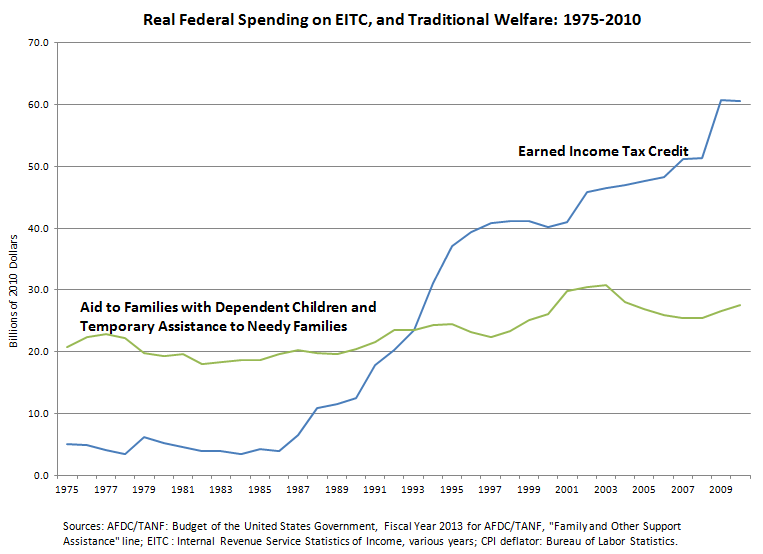
\includegraphics[width=0.9\textwidth]{graph.png}
\end{figure}

Even though tax expenditure spending should be viewed analogously to direct government spending, the politics between the two types of policy are often times quite different and possibly reactive to one another in a way not previously outlined in the literature. One illustrative example is the case of poverty in America. Building on a state run program to provide cash assistance to single mothers, Congress passed Aid to Dependent Children (ADC) which subsidized those state programs for that constituency. By the 1960s, through a series of eligibility changes enacted over the previous thirty years, ADC was the `most expensive' traditional welfare program in the country and served many more types of constituencies than just single mothers. As more Americans became eligible and started receiving ADC, it became increasingly unpopular among the public and elites and it was especially vulnerable to retrenchment in the early years of the Nixon presidency \citep{moynihan1973}. 

In 1974 and in spite of the desperately unpopular AFDC,\footnote{The program was renamed from Aid to Dependent Children to Aid to Families with Dependent Children during the Great Society period of the 1960s.} Congress quietly passed a refundable tax credit for the working poor. The Earned Income Tax Credit (EITC) was a wage subsidy for low income people that would zero out their income tax liability and if any of the reward remained, the federal government would send the recipient a check for the remainder. While ADC was never expanded again and ultimately replaced with a far different program, the Earned Income Credit, social policy through the tax code, was expanded both in eligibility and generosity several times in subsequent decades \citep{stewart1991, myles1997}. This is clearly seen in the above graph where the EITC explodes in cost relative to AFDC and AFDC remains basically stagnant once the EITC is introduced. The relationship between direct and non-traditional programs has not been  explicitly discussed in the literature yet we have much to learn from this sort of policy relationship (See \citet{hacker2002} for a strong counter example). Why did legislators abandon expansions of direct welfare spending? Why was there a steady uptick in EITC spending even though it did almost the same thing as the now stagnant visible spending? By examining the way interests assemble into coalitions under congressional constraints, we can better understand how related policies develop so differently.

While there was significant expansion in the rights of many Americans during the 20th century, much of the policy conflict dealt with direct spending, tax expenditures, and regulation \citep{pierson2007}. Over time, these services and policies layer upon one another because political contexts change, which open or close different policy streams, changing the relative effectiveness and impact of the tools used to create policy \citep{kingdon2011}. Sometimes policies are retrenched, as in the case of ADC, and sometimes policies grow and grow because other other avenues are closed off or political interests change. Additionally, that different tools create different types of policies, creates different politics. As illustrated above, the politics of visible programs may be radically different from the politics of tax expenditure programs. All of these factors come together to form the spending part of the `exceptional' American welfare state -- a disparate web of interconnected and sometimes competing policies which have layered over time and have been enacted through one of four distinct policy making mechanisms. Future research will need to keep broadening the scope of inquiry by including rights and while they are important in general, they are not included in this story. With that in mind, this dissertation deals solely with the spending parts of the policy. 

\subsection{Why Does American Social Policy Look This Way?}
Having briefly described the mechanisms that the government use to produce American social policy, we now turn to an overview of why and how the United States created and maintains this type of welfare regime. The United States has a fragmented welfare state with several different types of policy tools and policies. How did America reach that point? Most research on the American welfare state deals with hypotheses for why the United States has limited \emph{direct} social spending when compared to other developed countries while at the same time, largely overlooking non visible aspects of the welfare system. While imperfect, the explanations for the lack of visible social spending in the United States are a good start for discussing policy making overall. 

What is common to two of the three conventional wisdom theories of American welfare state development (the three being culture, labor, institutions) is that all identify political and economic interests which are translated into policy. For instance, one school of thought argues that the United States lacks visible spending because American elites and citizens do not want to have a `generous' welfare state \citep{king1973}. These scholars argue that public opinion and American political culture is not pro social spending so legislators are less likely to support advance social legislation. Another school argues that the interests of labor and business compete which results in social legislation being made or not \citep{korpi1980, swenson2004}. While these schools focus on the interests of groups, it is more likely that the preferences and strength of these groups fluctuates over time and even the groups themselves may not have monolithic preferences \citep{hacker2002b}. However, pure preferences are not flawlessly translated into policy -- preferences need to advance through an extremely complicated set of institutional barriers and arrangements to become policy \citep{pierson1995, robertson2011}. 

Even if the conventional wisdom provides great insight, it does not explain why the United States would choose to utilize one type of policy making tool. The United States has created lots of hidden policies before, in between, and after, the explosion of visible programs in the 1930s and 1960s yet we do not know why elites chose to use different policy making tools to accomplish their policy goals \citep[Ch. 2]{howard2008}. It is an important oversight that most conventional research on American social policy does not account for different ways of providing policy, instead focusing unilaterally on one of the four earlier mentioned mechanisms. It would be an excellent step to identify policies and policy tools as part of a broader choice spectrum where we examine the policy that was created against the alternative, un-enacted policies. For instance, to qualify for the Earned Income Tax Credit a person must have worked during the year while for a long time Aid to Dependent Children was an entitlement with no such working requirements. Now both programs have strong work requirements, while the minimum wage, even though it has been raised several times, has stayed at around the 1990 level in real dollars. In this way, the two main poverty alleviating policies force people into the labor market and push the cost of the program on the government. At one time, these programs had quite different politics but now they are very similar in many key ways which suggests a converging effect which is the trajectories of these programs together, even while the tax expenditure tool is more popular in general than direct spending \citep{faricy2014}. In short, there is great utility by examining the politics of policy choice rather than just the development of one policy.


\section{Towards a Holistic Understanding of Policy Making}
With that in mind, this dissertation will argue that the creation and expansion non-traditional spending vis-a-vis traditional welfare was largely a function of institutional and ideological constraints on legislators with different and sometimes competing motivations and preferences legislating around different and competing interests. The overtime fluctuations in legislator motivations and how members incorporate outside political interests into policy, against the backdrop of changes in the number of active veto points, institutional centralization, ideological polarization changes the type of coalitions which are possible, encouraging reliance on different policy making tools than in different situations. Under certain conditions, legislators will be able to advance a highly salient program, other times they may have to rely on less visible and less traditional programs to advance their goals. Put differently, the sort of winning legislative coalitions that are possible will coalesce around a social policy making tool which has the best prospect of becoming policy, under the constraints of the situation and the flexibility of the motivations of involved legislators.

This section outlines how the inputs and constraints of the legislative process encourage one type of policy to be made over another. First I discuss the goals of legislators, the way they advance them, and the effects this has on policy development. Second, I discuss the many way a legislator is constrained by macro level forces. Lastly, I combine both sections with the intent of setting up several expectations for the dissertation.

\subsection{The Flexibility and Multitude of Member Motivations}
Members of Congress, while constrained by institutions and other macro level forces, have their own individual level motivations, political preferences, and goals that they work towards advancing under those constraints. There are the basic goals mentioned by \citet{mayhew1974} and \citet{fenno1973}: re-election, prestige, and good policy but there are also several ways of achieving those goals. In pursing their goals, members will strive either try to claim credit or deflect blame in order to best serve their reelection interests if that is their most salient goal. This results in different types of policy tools being utilized based around different legislator goals \citep{weaver1986}. For instance, since the costs of proposed legislation are often targeted at certain groups while the benefits are often widely distributed, legislators may want try to deflect blame from the policy or advance a different type of policy. However, if a legislator can shift the policy debate to a different type of politics where, for what ever reason, the proposal is much less salient than the alternatives then a legislator may be able to get around the conflict with his or her constituency.

Additionally within the framework of legislators adopting blame avoidant or credit claiming strategies, highly salient programs are obviously more well known to constituents and so MCs are more likely to have a well developed opinion on the program or idea. This would encourage opposed MCs to step up their opposition in order to show constituents and other elites that they making good on opposing legislation they oppose. On the other hand, less visible programs are less salient to constituents vis-a-vis other policies with more prominence. This may allow MCs to have a less developed position on the program or not require them to be as staunch in their opposition as the constituents and other elites may not think to punish them for their lack of opposition. Overcoming passively opposed MCs is much easier than overcoming actively opposed MCs. Of course, policy visibility changes over time which would affect a given LE's preference structure and would open or close policy avenues as well. It may be that tax expenditures are one of the main forms of hidden policy now that may not necessarily be the case in the future as well. 


\subsection{The Changing Nature of Institutional Constraints}
The story of the post war American Congress is one of increasingly strict rules, a more powerful centralized leadership, and more ideological polarization \citep{rohde1991, binder2003}. Additionally, the mid 1970s saw the rise of a new brand of activist conservative who was more aggressive in attacking traditional welfare programs like AFDC were willing to attack institutional norms to accomplish their goals, and more willing to construct redistribution policy if it benefited their interests \citep{hacker2007, theriault2013}. The interaction of more centralized chamber leadership and more aggressive conservative members of Congress manifested itself in an increasingly hostile environment for traditional social policy. Additionally, conservatives became willing to use the levers of government to accomplish their own style of policy making. Any potential demand for federal assistance did not dissipate just because of this hostile environment, however, and many legislators still wanted to create and expand more expansive social policies. For some legislators, they found that they were able to quietly assemble a coalition of pro-business and certain pro-welfare policy makers to advance a tax expenditure which may have reduced costs to business while increasing social spending. 
 
In this subsection, I outline some of the macro institutional forces which specifically influenced the creation and expansion of non-traditional social policies while also discouraging the creation and expansion of traditional welfare programs. First, I describe the way key institutional processes have changed, including changes in congressional rules and behaviors over the last fifty years in both chambers of Congress while also noting the importance of other institutional constraints. Second, I outline how the rise of a new style of Republican learned to use government for their own policy and political means. Consequently and to reiterate, changes in institutional rules and individual preferences / tactics intersect to encourage policy makers to pursue one type of policy over another in a given agenda area.

From a broad stand point, the ebb and flow of centralized leadership in both houses of Congress is one of the most fundamental factors in encouraging different forms of policy making. During the creation of the New Deal and Great Society, leadership was in the hands of the committee chairs and much of the power rested with the bipartisan conservative coalition even though the Democratic technically controlled both Congressional chambers for much of this time \citep{shelley1983, shepsle1989, polsby2004}. In addition, many of the informal norms of the era were based on reciprocity and a strong seniority tradition \citep{matthews1960, asher1973}. As a result of these two forces, conservative southerners held much of the legislative power because they were the most senior and were able to rule their committees like little fiefdoms.\footnote{Though members who were not empowered in the committee centric system would try to circumvent these entrenched chairs via discharge petitions \citep{pearson2009}} One excellent example of this committee dominated landscape is that one of the House Rules Chairman in the 1950s, Howard Smith (D-VA), would let liberal legislation accumulate -- with legislation often needing a special rule to advance to the floor -- and when the backlog is sufficiently great he would tell House Leadership to pick 2-3 bills from the many to advance \cite[pg. 14]{polsby2004}. Additionally, the amount of independence and power given to subcommittee chairs was at the discretion of the Chairs and quite limited \citep{rohde1974}. This period of `decentralized leadership' where both chambers relied on reciprocity, and a strong seniority tradition along with powerful committee chairs lasted until the mid 1970s when Democrats started empowering centralized leadership at the expense of committee chairs.

House Democrats in the mid 1970s wished to ``make the people who held positions of power responsible to rank and file Democrats" \citep[pg. 26, quote spoken by Rep. Donald Fraser (D-MN)]{rohde1991}. In pursuing this institutional goal, Democrats passed several intra-party reforms which drastically increased the power of centralized leadership and subcommittee chairs. They stripped many powers from committee chairs and had them run for intra-party election to retain committee chairs. Additionally, many of the powers taken from the committees were placed within central party leadership. The logic behind the internal reforms was to empower the Democratic caucus as a whole and to remove the fiefdoms of deeply entrenched committee chairs. Instead of southern Democrats with lots of seniority setting the agenda, the caucus as a whole got to choose which policies would be advanced in a given Congress. By the 1980s, not only had committee chairs lost most of their powers, the House Democratic caucus began empowering House leadership to negotiate policy on their behalf instead of merely acting as the agent of the party's majority \citep{sinclair1983, palazzolo1992, sinclair1998}. The goals were largely policy based -- Democrats had been stymied on their policy goals for many years by the bipartisan conservative coalition. With the dis-empowerment of committee chairs and the empowerment of the Democratic caucus, sub-committees chairs and backbench Democrats, liberals were able to break the conservative coalition's hold on policy in the U.S. Congress

%maybe include graphs? Check the evernote
The transition from a committee based House of Representatives to centralized leadership, empowered by the party as a whole, had profound effects on visible policy making and maintenance. Previously powerful individuals were now unable to exert their previously significant clout to advance their own policy goals. As the institutional power dynamic shifted, so too did the type of macro level voting patterns. With the disabling of the conservative coalition, rates of bipartisan passage have slowly declined since the 1970s \citep{trubowitz2005}. Inversely, both the number of party line votes and party unity scores for those party line votes have increased rapidly in the same period. From a purely institutional level, these institutional changes may be the mechanism that a would be coalition leader looks at when trying to decide how best to pursue a policy making strategy given the constraints of the situation.

The 1970s House reforms were largely adopted and expanded by the Republicans when they won control of both Congressional chambers in 1994 changing the types of policies created. With the now firmly Speaker centric Congress, conservatives in Congress were able to use the reforms passed by liberal Democrats in the 1970s to their own advantage as well \citep{zelizer2007}. Those with an interest in social policy now faced an even more hostile set of empowered actors because conservatives controlled the chamber and were actively trying to cut welfare spending and taxes. Prior to the 1970s reforms, the decentralized nature of the House chamber and the lack of well sorted congressional parties encouraged bipartisan and ideologically diverse voting coalitions, allowing even minority party members to realistically pursue their policy goals \citep{poole1997}. The Republicans who swept into office in 1995 viewed themselves as ideological purists and were largely unwilling to compromise with the now minority Democrats \citep{hacker2006, theriault2013}. Combined with the largely centralized chamber power, Republicans were able to simultaneously pass deep cuts to traditional welfare programs and also discourage legislators who may have wanted to temper any welfare cuts by very skillfully utilizing the centralized leadership structure of the House \citep{aldrich2000}. 

In the Senate, the story is very much the same except it was the reciprocal norm of respect eroding \emph{alongside} the centralization of leadership but with a slightly different time line \citep{sinclair1986}. Since the late 1980s, individual senators have spent more resources empowering their party's leadership and those leaders began changing the Senate agenda to maximize inter-party cleavages while minimizing their own party's ideological differences \citep{lee2008}. An obvious consequence of this type of agenda control is that it encouraged ideological sorting among Senators to the point where all conservatives were in one party and all liberals in the other \citep{poole1997}. It was already difficult to pass legislation through the Senate due to supermajority and unanimous consent requirements, so as parties became more homogenized the cost of moving the status quo increased greatly \citep{koger2010}. Like in the House, the changing configuration of legislative constraints and the hyper partisan attacks on individual senators encouraged legislators to develop new ways to legislate -- namely, through the less visible and non-traditional policies.

Outside of individual chambers of Congress, changes in divided government add another potential set of veto points which may could make legislating difficult. Prominently, \cite{mayhew1990} argues that divided government has no real effect on `major' legislation passed in a given Congress. In this case, major legislation means highly salient legislation and by definition does not account for tax expenditures. Conversely, divided government has been mentioned as relevant to the creation of hidden welfare spending. \citet[Ch. 4]{howard2008} argues that divided government is associated with more hidden welfare policies being made as it is harder to pass visible legislation in a divided government situation. Since 1970, the United States has had unified government 30\% of the time compared to 70\% for the earlier part of the 20th century. Again, institutional configurations change, legislators need to find creative ways to assemble coalitions to advance their goals.

In addition to the pure institutional constraints, the changing nature of American conservativism also became a constraint for policy making, a way not fully realized previously. The rise of the modern American conservative movement came directly as a reaction to the New Deal and the Great Society, and the activist state more generally \citep{critchlow2007, zelizer2010}. In postwar America, the driving conflict between liberals and conservatives was over the scope and size of the federal government \emph{within} the confines of a New Deal style safety net. Broadly speaking, conservatives wished to retrench direct spending welfare programs and generally wanted the federal government to do less but most conservatives did not want to remove the safety net altogether. However, the nature and tactics of conservatives started to change in late 1960s with an increase of conservatives rejecting the ``New Deal Consensus." Republicans were now willing to attack the major tenets of the American welfare state \citep{teles2007, skocpol2007}.

These new style conservatives started getting elected to Congress and just as the 1960s and early 1970s saw a change in tactics among Congressional Democrats, so too did the 1980s see a change in tactics among Congressional Republicans. The Republicans elected to the House of Representatives in 1978 or later showed a distinctly more confrontational style than earlier Republicans. They were willing to utilize any form of House procedure to embarrass or undermine Democratic leaders and were totally unwilling to go along with the ``permanent minority" status that House Republicans had been relegated to during the post-war era \citep{theriault2013}. Whereas Republicans of older generations had reverence for institutional legitimacy, these new style Republicans were willing to destroy institutional legitimacy to gain political power. Slowly and through several successful high profile attacks on Democrats, Rep. Newt Gingrich gained power in the Republican caucus with rank and file Republicans eventually going along with his confrontational approach \citep{harris2006}. 

It was this type of conservative that took over Congress in the 1995 and Speaker Gingrich was able to utilize the reforms of the 1970s designed to empower the majority party and caucus to advance Republican policy goals \citep{roberts2003}. The Republican House caucus under Gingrich changed several House rules to enact preferred policy preferences from the Contract with America. Additionally, the further increase in leadership centralization allowed for ideologically extreme members of Congress to more efficiently oppose alternative or liberal legislation. With key leadership positions in the House of Representatives controlled by the `new' brand of conservatives and with the increases in ideological homogeneity, negative agenda control would totally stymie liberal policy innovation and allow for conservatives to implement their policy preferences. As with other changes described thus far, lawmakers who wished to advance social policies needed to both work with Republicans and take a different strategy. This applies to the Senate as well where confrontational Republicans who came up as procedural warriors under Gingrich in the House got elected to the Senate and rapidly started using the looser Senate rules to their advantage to drastically increase both actual polarization and the aggressiveness with which it was invoked \citep{lee2008, theriault2013}.

\subsection{Combining Inputs and Constraints}
The rise of confrontational and ideological conservatism combined with the changes of congressional behavior and rules, I propose, can largely explain the creation and expansion of the non-traditional welfare state. Legislatures produce outcomes according to inputs and constraints. As Congress changed so did the types of policy it produced. Coalition leaders and legislative entrepreneurs, keeping their goals and strategies in mind, reacted to the changes in the legislative constraints by utilizing different policy tools based on what best allowed them to either claim credit or deflect blame and the political / institutional constraints to achieve a winning coalition which ultimately advanced their goal. Through a rise of restrictive rules, centralized chamber leadership, increased obstruction, increased polarization, and increased ideological extremism, advancing traditional spending based social policy through the traditional policy making process became too politically costly for politicians. Assembling a legislative coalition which can pass both chambers (which in modern times are extremely ideologically polarized), overcome a filibuster, and get signed into law by a potentially hostile President is a daunting task. Legislators who still wanted to advance social policy needed to find other ways to achieve their goals. Consequently, politicians deliberately chose less visible policy making techniques because the coalitions that may assemble around those sort of policies may have less developed preferences on the specific policy proposal compared to other, more visible, iterations of that policy type in addition to having less visible costs at the onset. Similarly, by sidestepping highly visible versions of that policy type it may be possible to reduce the possibility of drawing protracted opposition from hostile members. To that end, in advancing less visible policy, often times through the tax code, legislators found a tool that did not require as much political capital to advance and was not even on the radar of most other members of Congress, relative to other issues. In other words, legislators found a tool that allowed them to circumvent the gridlock interval in a novel way \citep{krehbiel1998, binder2003}.

\section{Theoretical Expectations}
The general argument of this dissertation is that the ideological polarization of a given time combined with institutional constraints of a given time, including chamber leadership centralization, divided government, and certain `pivots' such as the filibuster `pivot', produce different types of social policy based around legislator motivations and how they pursue those motivations. The strategies that policy makers use to ``overcome" the gridlock interval at a given time, which is difficult to begin with in American politics, change based on the way with which the interval is engaged. To that end, legislators choose to pursue policies that may be less salient than other policy alternatives because the less salient proposals may have a greater likelihood of overcoming the institutional barriers to change.

With that in mind, there are two sets of more specific theoretical expectations that I have in pursuing this dissertation. As the argument relies both on changes in institutions and also political actors, it makes sense to outline specific expectations for both components of the argument. In this section, I outline several expectations concerning the development and creation of both traditional and non-traditional welfare programs as a function of both institutional and individual factors. Consequently, I delve into when we can expect one type of policy tool to be used more often than a different tool.

One thing to note moving forward is that while this dissertation will use multiple methods, it will still attempt to make predictions of when some types of social policy would be made over others. Constructing expectations with actual predictions is especially important in a multi-methods style dissertation that may rely less heavily on traditional statistical analysis to ensure that scientific rigor is maintained. I will speak more to this later, but it is not the intent of this dissertation just to construct a narrative about social policy making in the United States -- it strives to understand under what conditions America produces and or expands one form of policy over another.

\subsection{Institutional Expectations}
I expect the most important institutional factor to be the centralization of chamber leadership. Holding other things constant, I expect more hidden and non traditional policies to be created when leadership is more centralized and further expect more visible and traditional social policy to be created when the legislature is less centralized. When coalition leaders design policies which appeal to the party median rather then the chamber median, there is less (if any) reason for minority party members to go along with the policy. While there is minimal reason for minority party members to go along with the majority party (see \citet{cox2004} for instance), many of the major traditional welfare programs had bipartisan coalitions for final passage even if they were more moderate than proponents may have wanted. Additionally, when leadership is centralized and party is emphasized, this highlights the cleavages between parties in a more stark way than in a decentralized Congress. With party being emphasized there is a stronger incentive for members to act as a partisan which may increase the level of conflict between the parties, resulting in more hostile relations and hardening opposition to policy along partisan lines with respect to existing political situations \citep{lee2009}. In having to overcome this sort of opposition, legislative entrepreneurs will attempt to advance less visible policy in both expanding existing programs and trying to create new hidden programs. 

A second institutional expectation is that when holding other things constant, a given Congressional chamber is more polarized, non traditional policy will be advanced. This is the most intuitive of expectations as polarization discourages policy making in general which would decrease the likelihood of advancing highly salient unless the majority party is extremely large. Trying to overcome a polarized legislature is difficult so legislative entrepreneurs will try to advance policies which are least likely to draw solidified opposition.

Moving away from intrabranch issues, I expect that divided government of all types will encourage non-traditional policy making and expansion, while more unified government will encourage traditional policy creation and expansion. While there is disagreement as to the role of divided government in passing legislation in general, we do not know how divided government changes the type of policy enacted into law. In times of divided government, legislators who wish to advance policy goals need to potentially overcome more engaged veto points so they have to resort to hidden policy making tools. During times of unified government, the government is incentivized to pass visible policy so they can claim credit for electoral benefits.

Additionally, I expect governing party durability to be an important factor in visible policy durability but not as important for hidden policy durability. \citet{berry2012} argues that policies are more likely to be retrenched if the party that enacted the policy loses seats in following the enactment. I expect this pattern to apply more to traditional policy because a new, potentially hostile regime is more aware of a visible policy, because it is by definition the type of policy people know about. As newer coalitions may be less informed of a less salient policy than they are of visible policies when they are first elected, I expect those policies to survive coalition changes more easily. 

One thing to note at the onset is that all of the forces outlined in this proposal intersect but that is especially true for the institutional forces. While it may be prohibitively difficult to outline my expectations for every interaction at this stage, there are two interactions where I have have expectations. First, I expect that in situations with a very centralized and polarized Congress, operating in a fully unified government (including a 60+ member Senate), we would see much more traditional policy being advanced and/or non-traditional policies that previously had been `hidden' being revealed and advanced. The reasoning is that electorally, the governing party has to show that it can pass an agenda and it is much easier to claim credit for widely known policies. A second interaction based expectation is that when polarization high and chamber leadership is centralized, we will see increased importance of the filibuster pivot, creating a very high bar to advancing legislation \citep{koger2010}. Under those circumstances, I would expect policy making to decline overall unless the situation is similar to the one outlined in the first interaction, but I would expect much of the policy that does to be of the less visible variety.

\subsection{Actor Based Expectations}
While institutional constraints and active institutional veto points are important, so are the people who wield the levers of government and attempt to advance as well as oppose social policy creation and expansion. Trying to determine actor based factors are relevant to social policy creation and expansion is difficult but it can roughly be broken down into two types of MCs: the legislative entrepreneurs who seek to pass and expand social policy and those who oppose such efforts. This section outlines expectations for both groups.

One assumption of my argument is that less salient policies are pursued because they are less costly politically however that is not true for every member equally. To pursue such a legislative strategy requires the information to know about the policy tool, political power to use such a tool, and ultimately exploit the tool successfully. With that in mind, I expect that the legislative entrepreneurs who are primarily responsible for hidden policy creation and expansion to be disproportionately powerful, senior, and electorally safe MCs. The reasoning for this is that I expect to find many hidden programs are created or advanced by last minute amendments or additions to committee reports or floor bills. It would be much easier for people who chair the relevant committee or who have seniority to attach such an amendment without drawing scrutiny from other members. A less experienced member would most likely draw scrutiny with this type of behavior or choose not to do it for other reasons. Additionally, members who are focused on creating public policy are probably willing to care less about the  policy making strategy, preferring to focus on the outcome \citep{weaver1986}. This is in line with the idea that these sort of members advance legislation that is harder to claim credit for in the electoral arena, sometimes to their demise \citep{hibbing1991, wawro2001}.\footnote{Even though \citet{wawro2001} shows that there is no link between re-election benefits and legislative entrepreneurship, the idea that MCs pursue their goals differently and use policy to achieve reelection is not new \citep{fenno1973, kernell1999}. To that end, I assume that a legislator who is trying to rely on policy advancement for election would focus on high profile legislation even if there are minimal tangible benefits.} 

Trying to make a set of predictions for who tries to advance visible legislation is difficult since that would presumably be the default way for most members to advance legislation. Every Congress there are tens of thousands of pieces of legislation introduced so how can we derive systemic predictions about who sponsors the default type of legislation? In general, I would expect that major visible policy ideas to be sponsored by the same type of MCs who seek to advance less salient policy just under the institutional constraints that allow for visible policy creation. \citet{wawro2001}'s analysis of legislative entrepreneurship points out that there is a limited relationship between policy making and re-election based activities so it would be plausible to think that LEs care less about re-election or are safe in that arena. Additionally, \citet[Ch. 3]{evans2004} notes that coalition leaders are often committee leaders who are in the position to offer some form of pork in the course of forming a policy coalition -- implying someone senior and powerful. 

Once a hidden policy is enacted into law, I expect the individual level requirements for expansion of that program to ease, all things considered. The rationale is that as a policy remains relatively hidden, any potential political conflict surrounding the policy is largely preempted which preempts organized attempts to retrench such a program. However, If a hidden program becomes more visible or a visible program becomes even more visible, I expect the individual level political capital costs to increase. If a program is highly visible then members who wish to expand the program must overcome potentially active veto points in a way that would be similar to any typical visible policy.

While those who seek to create and expand social policy are an important set of actors, also important are the individuals who oppose social policy advancement. I expect that the rise of activist conservatives in the 1980s, will result in Republicans more forcibly engage in active policy making instead of just trying to oppose Democratic spending. For instance, Republicans advanced one of the largest expansions to Medicare ever with the prescription drug coverage. While it drastically increased the federal commitment to seniors, it also was a very large subsidy for drug companies. Additionally, while Republicans have gotten a reputation for opposing the Affordable Care Act, their targeted opposition helped shape it in such a way that private insurers were subsidized through the legislation. The type of policy being created once the Republicans started forcefully using their positions to benefit their constituencies.

\section{Research Design}
%include more formal language about independent variables, quantative context, role of CC
% can create a model of coalition types passing with the congressional bills package.
The body of the dissertation will be based around the creation and historical development of six individual policies within two separate goal areas of social policy, cash assistance and housing policy. This strategy has numerous benefits. One such being that this strategy allows a research design which combines both within-case and cross-case comparison in a unique two level way \citep{george2005, goertz2012}. As described in Table One, by treating individual policies as cases we are able to examine how institutional and actor changes affected a given policy over time, allowing for within-case analysis. At the same time, we are able to trace individual policy creation development in relation to other policies in the same policy area, allowing for cross-case comparisons. Similarly, when we treat policy area as the unit of analysis, we can examine how a policy area changes over time and how policy areas developed in relation to one another. By using this type of case study approach, I am able to develop a very flexible broad based approach to this dissertation where we can see how policies and policy areas developed and changed in response and alongside one another. 

%lol this table looks super bad in code. Don't ever change it.

\begin{table}
\centering
    \begin{tabularx}{\textwidth}{XXX} \toprule
           & \textbf{Within Case Comparison} & \textbf{Cross Case Comparison                                                                              } \\ \midrule
    \textbf{Individual Policy Level} & Trace Creation and Development of Individual Policies        & Compare Creation and Development of Individual Policies against other policies within a policy area \\
    \textbf{Policy Area Level}       & Trace Creation and Development of Policies in a Policy Area as a Whole & Compare Creation and Development of Policy Areas against other Policy Areas                         \\ \bottomrule
    \end{tabularx}
  \caption{Multi-Level Case Study Design}
  \label{tab:casestudy}
\end{table}

Those six policies used for this dissertation, described in table two, are representative of the type of spending policies that politicians choose to utilize in providing social policy. In selecting policies to analyze, one must be careful to ensure the method of policy making represents a wide swath of options available to policy makers. Considering this, I have chosen policies within a goal area to represent the array of individual policies a politician may choose to advance their policy goal. Since legislators care about policy goals, they will choose whatever tool allows them to advance that goal. The three policies per goal represent those options. 

Additionally, the goal areas and individual policies are often times what people mean when they say welfare which allows for external validity. Much of the previous literature on welfare state creation and maintenance deals with health care policy or pension policy, but there is less scholarship on cash assistance or housing \citep{derthick1979, hacker2002, campbell2005}. To be sure, they are well studied policies but we only understand them on an individual level basis. As such, do not know why, for instance, we would see an expansion in one type of cash assistance (EITC) but not another (AFDC). These goal areas lead themselves to this type of analysis very well.

\begin{table}
\centering
    \begin{tabularx}{\textwidth}{XXX} \toprule
           & \textbf{Housing Policy} & \textbf{Cash Assistance Policy} \\ \midrule
    \textbf{Traditional Social Policy} & Public Housing        & Aid to Families with Dependent Children \\
        \textbf{Mixed Social Policy} & Housing Choice Voucher Program        & Supplemental Nutrition Assistance Program \\
    \textbf{Tax Based Social Policy} & Home Mortgage Interest Tax Deduction        & Earned Income Tax Credit \\ \bottomrule
    \end{tabularx}
  \caption{Types of Policies According to Policy Tool Area}
  \label{tab:types}
\end{table}

From a broad stand point, this dissertation will examine both macro trends in social policy making and maintenance along with trends in individual policies within two distinct social policy goal areas. In pursuing that strategy, this dissertation will use a combination of quantitative and qualitative methods in order to make it's case that certain changes in institutions and behaviors encourage one type of social policy making over another. Additionally, this dissertation will extend over a wide swath of the 20th and 21st century enabling the ability to examine changes in social policy making against the backdrop of changes in the congressional behavior and institutions.

More specifically, this dissertation will use both quantitative and qualitative methods and data. At every step of the way, I hope to combine both a qualitative and historical narrative punctuated with sophisticated statistical analysis. Quantified measurements of interest such as program visibility will be utilized throughout. The dissertation will begin with a quantitative examination of visible versus hidden social policy trends over the last several decades, showing that visible policies have stagnated (or declined) while hidden policies have exploded. This presents the empirical puzzle, sets the stage for subsequent analysis, and also continues to fill the gap in American social policy literature by showing that substantial parts of the American welfare system are distributed through the tax code. Additionally, it helps show that the growth of more visible polices are in a dynamic relationship with hidden policies where policies might change in reaction or in tandem to one another. By pairing the larger spending analysis with two large scope case studies, we create a methodological strategy where we examine the same policies and politics through different lenses, bringing even more insight.

As with the overview section, analysis of the case studies and policy goals will use both quantitative data alongside qualitative data. The role of constructing a narrative is important in the case studies because it will allow us to highlight relationships not easily uncovered with traditional data analysis. When dealing with such large stretches of history -- in one case back to at least 1913 -- with many different moving parts, it makes sense to tell the theoretical story qualitatively and provide quantitative evidence at key points in the story. Most importantly, if I am to make predictions about the sort of policy that that will be created I need a body of evidence to draw upon. I envision using the following types of data to help provide this evidence:
\begin{itemize}
\setlength{\itemsep}{-5pt}
\item Roll call vote data
\item Cosponsor data
\item Bill characteristics data including sponsor characteristics, how far the bill advanced, number of cosponsors.
\item Committee vote data
\item Speech data including non legislative speech, debate speech, committee speech
\item Roll Rates
\end{itemize}
These data are the quantified outcomes of what happens in Congress on a day to day basis. Broadly, these data allow us to measure individual level behaviors in a party controlled environment. We are looking for both how the institutional constrains the actor and how the actor overcomes (or does not) those constraints. For instance, do we see that a very senior member is rarely on the losing side of a floor vote and has high level traits of being a legislative entrepreneur? That member might be a strong candidate for someone who advances hidden legislation. Do we see a member who routinely gives bombastic speeches on the House Floor, is often on the losing side of a vote, and does not get many cosponsors for their proposals? That member might be the sort of member that exacerbates polarization and engages veto points, forcing other members to pursue different policy making strategies.

Additionally, many of the hypotheses require proxies for relevant quantitative analysis. As I outlined earlier, I expect that the most important forces will be Congressional leadership centralization in both chambers, legislative polarization, divided government, governing party durability, ideological extremism, the filibuster pivot and policy visibility. Some of these are relatively easy to develop measurements to use in the dissertation. Ideology, for instance, is generally measured by using NOMINATE scores \citep{poole1997}. Different divided government regimes can be noted as dummy variables. The more difficult proxy to identify is a measurement of centralization  of leadership. One strategy would be to just use polarization as a proxy, building off of the conditional party government idea that as Congressional parties become more polarized and homogeneous they strengthen central leadership \citep{rohde1991}. This approach would tell an oversimplified story and is riddled with endogeneity problems. Another strategy, which is the strategy I think will be best, is to survey the literature on leadership power in a given Congress and systematically but subjectively construct a measurement for how centralized the leadership is for that congress, and repeat until I have developed a measurement for all the congresses of interest. In pursuing that strategy for constructing the centralized chamber measurement, I rely on two sources, \citet{binder1997} and \citet{schickler2001}. \cite{binder1997} and \cite{schickler2001} outline explicit institutional changes which result in Congressional power dynamics with \citet{binder1997} focusing on the ebb and flow between majority and minority powers and \citet{schickler2001} dealing with that in addition to changes in intraparty strength as well. In both these pieces, they examine the way formal rules change to strengthen various interests in Congress. By incorporating their evidence and arguments, a strong measurement of leadership centralization could be made that is well grounded in previous Congressional literature.

Another specific measurement I'll have to construct is policy visibility. This allows me to examine the way policy alternatives ebb and flow into the agenda and out of the agenda. My version of visibility also has the ability to change over time which means a grounded measurement is required. For measuring program visibility to elites, I will construct a relative measurement based on the Policy Agendas Project data which has categorizes legislation according to the policy content of the legislation \citep{baumgartner2009}. The categorization scheme involved in this data is very fine grained and will allow for a very good temporal comparison in agenda changes of my policy cases and possibly even policy goals as well. In measuring how visible policies are to elites, I am not making the claim that members are ignorant of policies, but I do think that relative differences in salience between policies can make a big different in opposition or likelihood Program visibility to regular people would measured by newspaper articles from both liberal and conservative newspapers \citep{segal2002, gentzkow2010}. Many major newspapers make their archives public for large swaths of time so it would be relatively easy to construct a measurement of relative policy visibility across large spans of time. By using newspapers of differing ideological persuasions (and newspapers in general) we are able to see how much attention was paid to the policy cases in this dissertation.

One drawback to this style of research design is that it relies on a collection of data sources, narratives, and interpretation to develop the argument. While in many ways it may be a strength to build a case upon a collection of sources, such a strategy lacks scientific rigor in the traditional sense \citep{king1994}. Regardless of these claims, it is more difficult to find causal links with this sort of research design than it might be with a less ambitious set of arguments, thus raising the bar for making the claims this dissertation hopes to make. By intentionally designing the dissertation in this way, hopefully the this produces a better document overall which persuades more people I am able to overcome the higher threshold of causality.

Regardless of the relative merits of the research design, I envision it being relatively similar to both \cite{zelizer1998} and \cite{schickler2001} in tandem. \cite{zelizer1998} examines the structural constraints on long time House of Representatives Ways and Means Chairman Wilbur Mills and how they shaped the types of policies he pursued (and also his attempts at changing the constraints). Zelizer is an academic historian so his book is largely concerned with constructing a narrative about Mills and these constraints through time. I am looking at the question of choosing which legislative tool through the same sort of lens. Some constraints encourage different behavior and politicians react accordingly. Additionally, \cite{schickler2001} tells a story about how diffuse interests come together at different points in Congressional history to change the institutional rules and constraints. His work is largely historical in outlook as well, but he shows the effect of some of those interests using traditional quantitative analyses such as regression. I anticipate that sort of strategy will be extremely helpful towards my dissertation.

Overall, the research design for this project is flexible enough to account for many covarying parts while remaining powerful enough to tell a causal story. By combining a multitude of primary, secondary, quantitative and qualitative data sources I will be able to weave a strong multi-methodology dissertation which does not rely too heavily on one particular analysis to make an argument. Additionally, by using several different units of analysis, this dissertation will be strongly positioned to isolate relevant causal factors in the pursuit of identifying reasons why MCs choose to advance one form of policy over another. An additional benefit to that form of research design is that it strongly positions the dissertation to tell a readable and compelling narrative to underlay the analyses in the document. 


\newpage
    \bibliography{EITC}{}
\bibliographystyle{jpe}

\newpage
\appendix
\section{Tentative Chapter Outline}
I originally did not include this because I was and am having a difficult time imagining a broad structure. I think having a starting place is better than not, however, so I have added one. My main concern is that I am having trouble trying to balance substantive chapters with methodological / secondary chapters. This current setup has an introduction chapter, a conclusion chapter, two case study chapters, and a methodology chapter. I am not sure if there is enough weight to the substantive chapters.

\begin{description}
\item[Chapter One] The first chapter would introduce the puzzle and overview the theory. In the first part of the chapter, I will argue that there is tremendous value in combining the literature concerning Congress with the social policy literature. Specifically, I will introduce the idea that members have individual goals and several ways they choose to pursue those goals but individual members are constrained by institutional constraints. In conjunction, I will also introduce that when trying to form policy coalitions, the different goals (and ways members pursue them) come together in potentially interesting ways both by proponents and, for lack of a better term, opponents of a proposal.

From there, I will pivot to presenting the two broad `agenda items' in housing and income support and show how insight from the Congressional literature can help illuminate why one type of policy gets made over a different type in a given agenda item. I use the two broad policy areas to show how certain factors, either individual or institutional, that produce one type of policy over another.

\item[Chapter Two] I think the second chapter would be a broad research design chapter and hypotheses chapter. It seems like my research design and case selection especially is relatively complex and may benefit from explicitly laying out how I picked the cases, how I am going about trying to show causality, and how I am utilizing mixed methodology. For instance, I think a part of this chapter can be comparing across case area to explain how the three policy types I choose to represent an agenda item to show some form of external validity in proving that these are broad representations of how Congress creates policy. Likewise, I could discuss policy proposals within an agenda area to show an internal validity for that policy area. I think this would fit nicely with a discussion as to how the Congressional components introduced in chapter one intersect with the research design to create my guiding expectations and hypotheses in the substantive chapters.
\item[Chapter Three + Four] One of the these chapters would be a chapter about how Congress produces housing policy and the other would be about how Congress produces income support policy. A given chapter would involve discussion about how the Congressional aspects mentioned in chapters one and two play their part at choosing policy make up, which interests are included in a policy and which are left out at both critical junctures and policy maintenance. 
\item[Chapter Five] Conclusion Chapter.
\end{description}

\newpage
\section{Legislative Histories}
\begin{figure}[h!]
  \centering
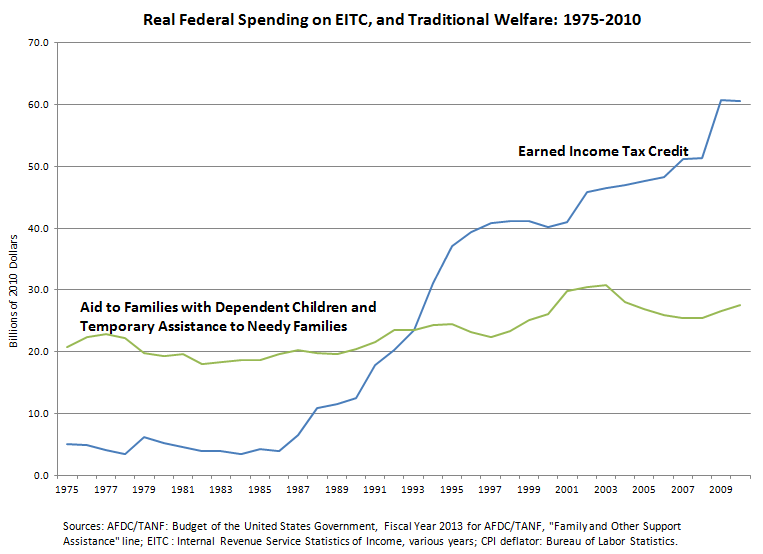
\includegraphics[width=0.9\textwidth]{graph.png}.
\end{figure}
\subsection{Earned Income Tax Credit}
Adopted from \citet[Appendix 1]{scott2007}.
\begin{description}
\setlength{\itemsep}{-5pt}
\item[1976] Policy Enacted
\item[1978] The EITC was made permanent (before it had to be renewed yearly) and maximum benefit raised
\item[1984] Maximum credit raised
\item[1987] The program became indexed to inflation, maximum credit raised again 
\item[1990] Maximum Credit raised and began adjusting upward for number of children in family
\item[1993] Maximum credit raised, extended eligibility to ``Childless Households''
\item[1994] Extended eligibility to American families living abroad.
\item[1995] Begins counting investment income as income for purposes of EITC
\item[1996] Increases what counts as income for purposes of EITC, denies benefit to undocumented workers, broadens income used in EITC phase out, and allows states to count EITC as income for state level welfare programs.
\item[2004] Allowed soldiers to count combat pay as income
\item[2008] Temporarily expanded EITC benefit
\item[2010] Reauthorized temporary benefit expansion
\end{description}

\subsection{Aid to Dependent Children}
Adopted from \citet[Appendixes A and B]{mittelstadt2005} and \citet{bell1965}.
\begin{description}
\setlength{\itemsep}{-5pt}
\item[1935] Policy Enacted
\item[1939] Increased benefit, split off some ADC recipients into Old Age and Survivors Insurance
\item[1952] Increased federal matching part of program and maximum amount for certain recipients
\item[1956] Stated goal of ADC changes from providing income support to encourage individual support
\item[1960] Bureau of Public Assistance asserted that states who refuse funding to `illegitimate children' would lose ADC funding.
\item[1961] Allowed for children of unemployed parents to become eligible for ADC in addition to the traditionally eligible groups and created work training program to employ the unemployed parent
\item[1962] Name changed to AFDC, increased job training funding
\item[1967] The Work Incentive Program required that most unemployed AFDC recipients be referred to jobs (obstinately to create jobs).
\item[1971] Increased number of unemployed AFDC recipients required to participate in work programs
\item[1996] AFDC replaced with TANF
\item[2012] Department of Human Services begins allowing states to apply for waivers to remove work requirement provision if they can meet certain benchmarks.
\end{description}


%\printbibliography
\end{document}

